\documentclass{article}
\usepackage{amsmath}
\usepackage{amsthm}
\usepackage{enumerate}
\usepackage[bookmarks=true]{hyperref}
\usepackage{bookmark}
\usepackage{graphicx}

\newif\ifALL

\ALLtrue

\usepackage{amssymb,amsmath,amsthm,amsfonts}
\usepackage{mathrsfs}
\usepackage{dsfont}
\usepackage{enumerate}

%\newtheorem{mdef}{Definition}
%\newtheorem{theorem}{Theorem}
\newcommand{\eqsplit}[2]{
  \begin{equation}\label{#2}
    \begin{split}
      #1
    \end{split}
  \end{equation}}
\newcommand{\eqnsplit}[1]{
  \begin{eqnarray*}
    #1
  \end{eqnarray*}}
\newcommand{\tran}[1]{
  \tilde{#1}
}
\newcommand{\td}[2]{
  \frac{d #1}{d #2}
}
\newcommand{\pd}[2]{
  \frac{\partial #1}{\partial #2}
}
\newcommand{\ppd}[2]{
  \frac{\partial^2 #1}{\partial #2^2}
}
\newcommand{\pdd}[3]{
  \frac{\partial^2 #1}{\partial #2 \partial #3}
}
\newcommand{\otd}[1]{
  \frac{d}{d #1}
}
\newcommand{\opd}[1]{
  \frac{\partial}{\partial #1}
}
\newcommand{\oppd}[1]{
  \frac{\partial^2}{\partial #1^2}
}
\newcommand{\opdd}[2]{
  \frac{\partial^2}{\partial #1 \partial #2}
}
\newcommand{\ket}[1]{
  |#1\rangle
}
\newcommand{\bra}[1]{
  \langle#1|
}
\newcommand{\inn}[1]{
  \langle#1\rangle
}
\newcommand{\mean}[1]{
  \langle#1\rangle
}
\newcommand{\tr}{
  \text{tr}\,
}
\newcommand{\re}{
  \text{Re}\,
}
\newcommand\im{
  \text{Im}\,
}
\newcommand{\var}{
  \text{var}
}
\newcommand{\arcsinh}{
  \sinh^{-1}
}
\newcommand{\arccosh}{
  \cosh^{-1}
}
\newcommand{\erfc}{
  \text{erfc}
}
\newcommand{\E}{
  \mathbb{E}
}
\renewcommand{\P}{
  \mathbb{P}
}
\newcommand{\I}[1]{
  \mathbf{1}_{\{#1\}}
}
\newcommand{\1}[1]{
  \mathds{1}_{\{#1\}}
}
\newcommand{\diag}{
  \text{diag\,}
}
\newcommand{\M}{
  {\text{max}}
}
\newcommand{\m}{
  {\text{min}}
}
\newcommand{\ph}{
  {\text{arg}\,}
}
\newcommand\erf{
  \text{erf}
}
\renewcommand\vec[1]{
  \mathbf{#1}
}
\newcommand\mtx[1]{
  \mathbf{#1}
}
\newcommand\ed{
  \,{\buildrel d \over =}\,
}



\title{On FX Rates and a Multivariate GARCH model}
\author{Xie Xiaolei}
\date{\today}
\begin{document}
\maketitle

\section{Notation}
We study the covariance matrix of a $p$-dimensional sequence with each
component modeled by a GARCH(1, 1) process:

\begin{eqnarray*}
  X_{i,t} &=& \sigma_{i,t} Z_{i,t} \\
  (Z_{1, t}, Z_{2,t}, \dots, Z_{p,t}) &\sim& N(0, \Sigma) \\
  \sigma_{i, t}^2 &=& \alpha_{i,0} + \alpha_{i,1} X_{i, t-1}^2 + \beta_{i,1} \sigma_{i, t-1}^2
\end{eqnarray*}

\section{Spectra of S\&P sectors}
\subsection{Utilities}
Fitting the daily returns' data of 25 companies that have been
included in the S\&P 500 index since 2010-01-01 and categorized in the
sector ``Utilities'', we obtained 23 GARCH(1, 1) models that satisfy
the condition
\begin{equation}
  \label{eq:garch_cond1}
  \alpha_1 + \beta_1 < 1  
\end{equation}
Then we simulate the GARCH(1, 1) processes with innovations having the
same covariance structure as those of the real data. Figure
\ref{fig:Utilities_eigenvalues} and \ref{fig:Utilities_eigenvectors1},
\ref{fig:Utilities_eigenvectors2}
compare the eigenvalues and eigenvectors, respectively, of the 
covariance matrices of the real and the simulated data.
\begin{figure}[htb!]
  \centering
  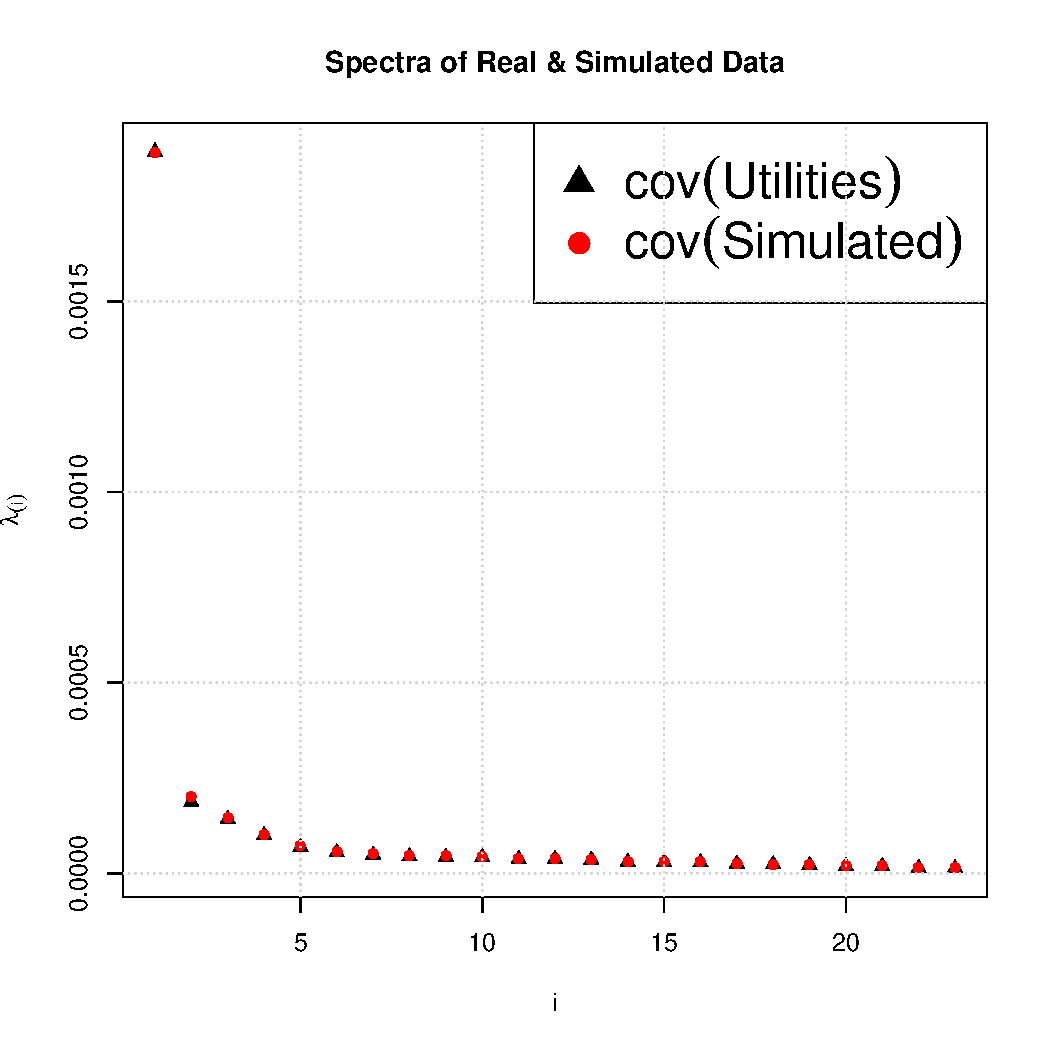
\includegraphics[scale=0.6]{Utilities_eigenvalues.pdf}
  \caption{Eigenvalues of Utilities: real \& simulated}
  \label{fig:Utilities_eigenvalues}
\end{figure}

\begin{figure}[htb!]
  \centering
  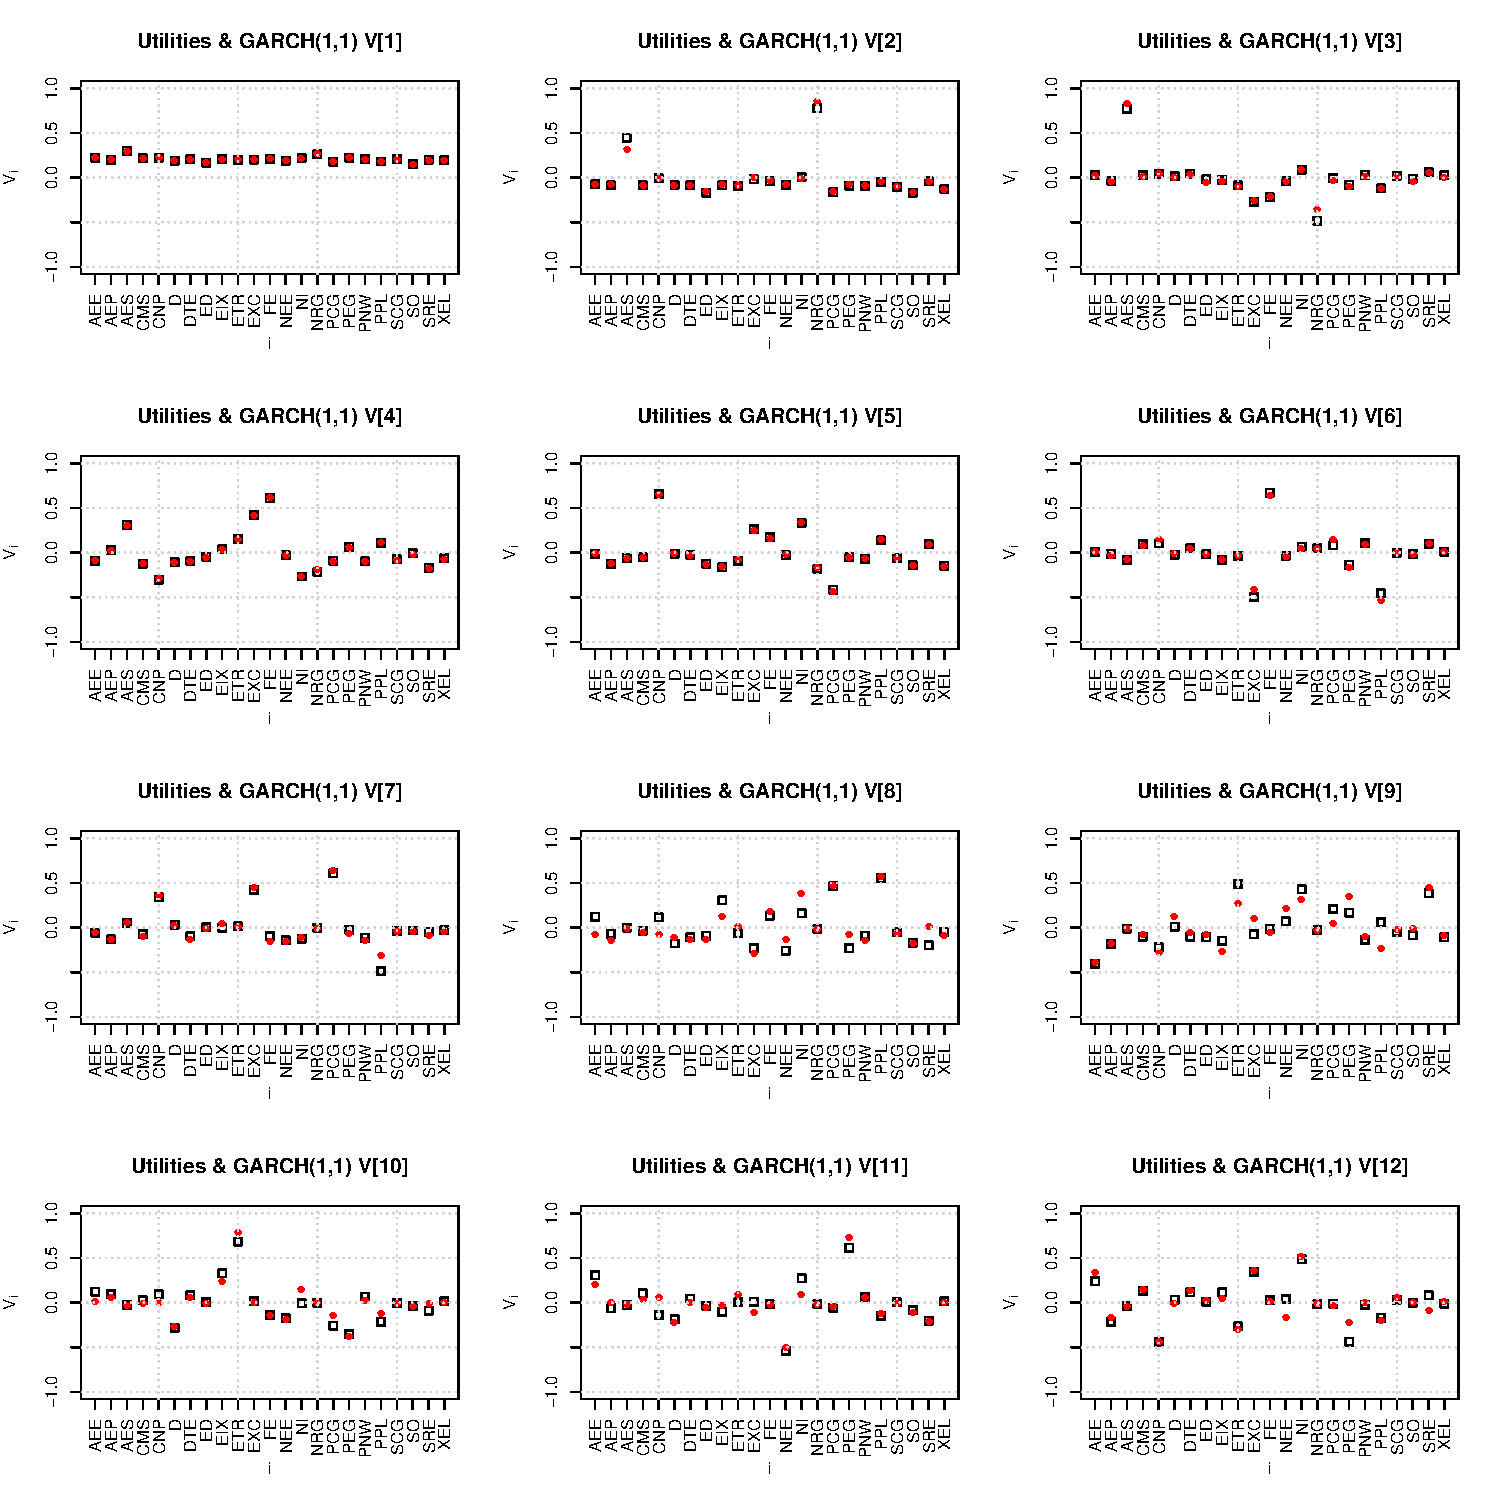
\includegraphics[scale=0.5]{Utilities_eigenvectors1.pdf}
  \caption{Eigenvectors of Utilities: real \& simulated}
  \label{fig:Utilities_eigenvectors1}
\end{figure}

\begin{figure}[htb!]
  \centering
  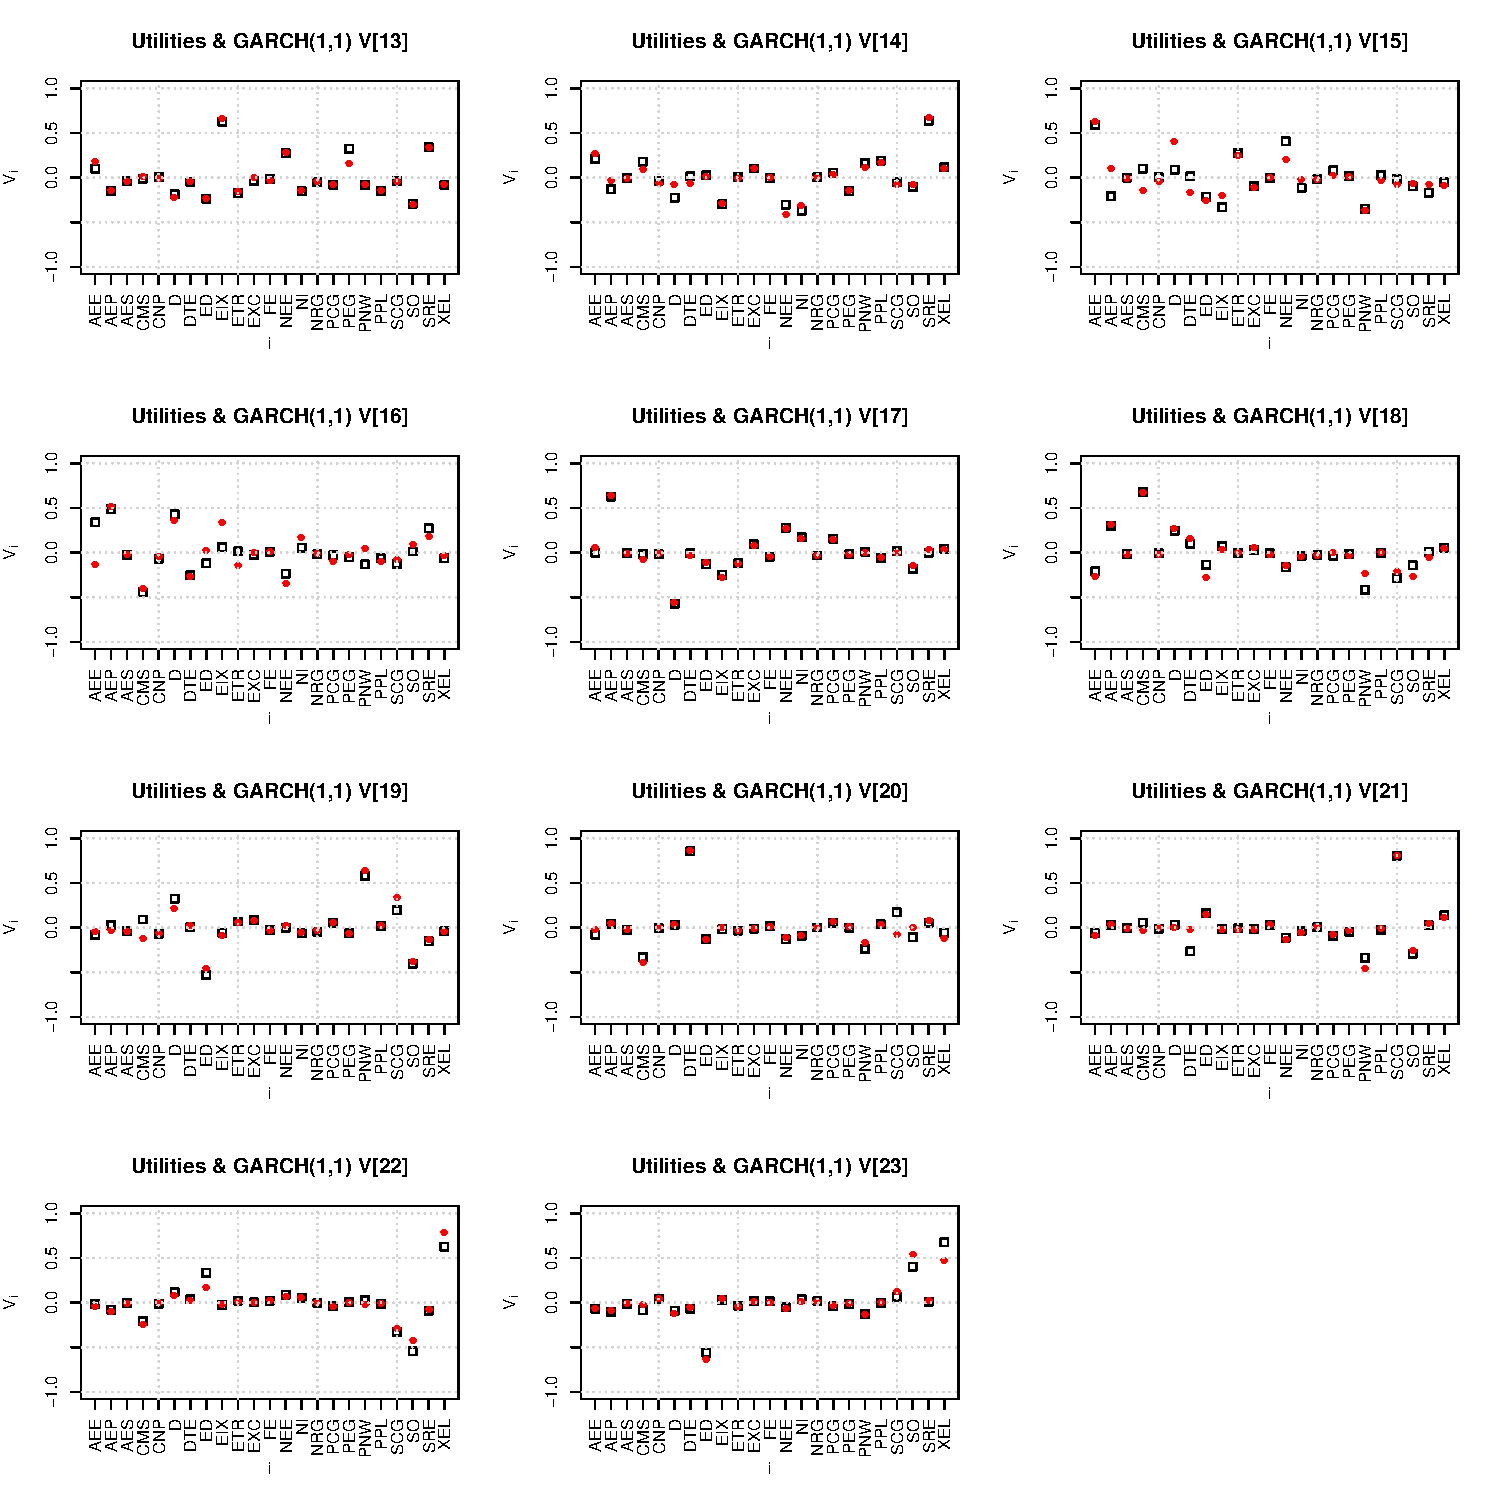
\includegraphics[scale=0.5]{Utilities_eigenvectors2.pdf}
  \caption{Eigenvectors of Utilities: real \& simulated continued}
  \label{fig:Utilities_eigenvectors2}
\end{figure}

\subsection{Materials}
A similar analysis on the ``Materials'' sector produces the following
spectra. In this sector, 21 out of 25 return sequencies are
successfully fitted to GARCH(1, 1) models that satisfy condition
\eqref{eq:garch_cond1}.

\begin{figure}[htb!]
  \centering
  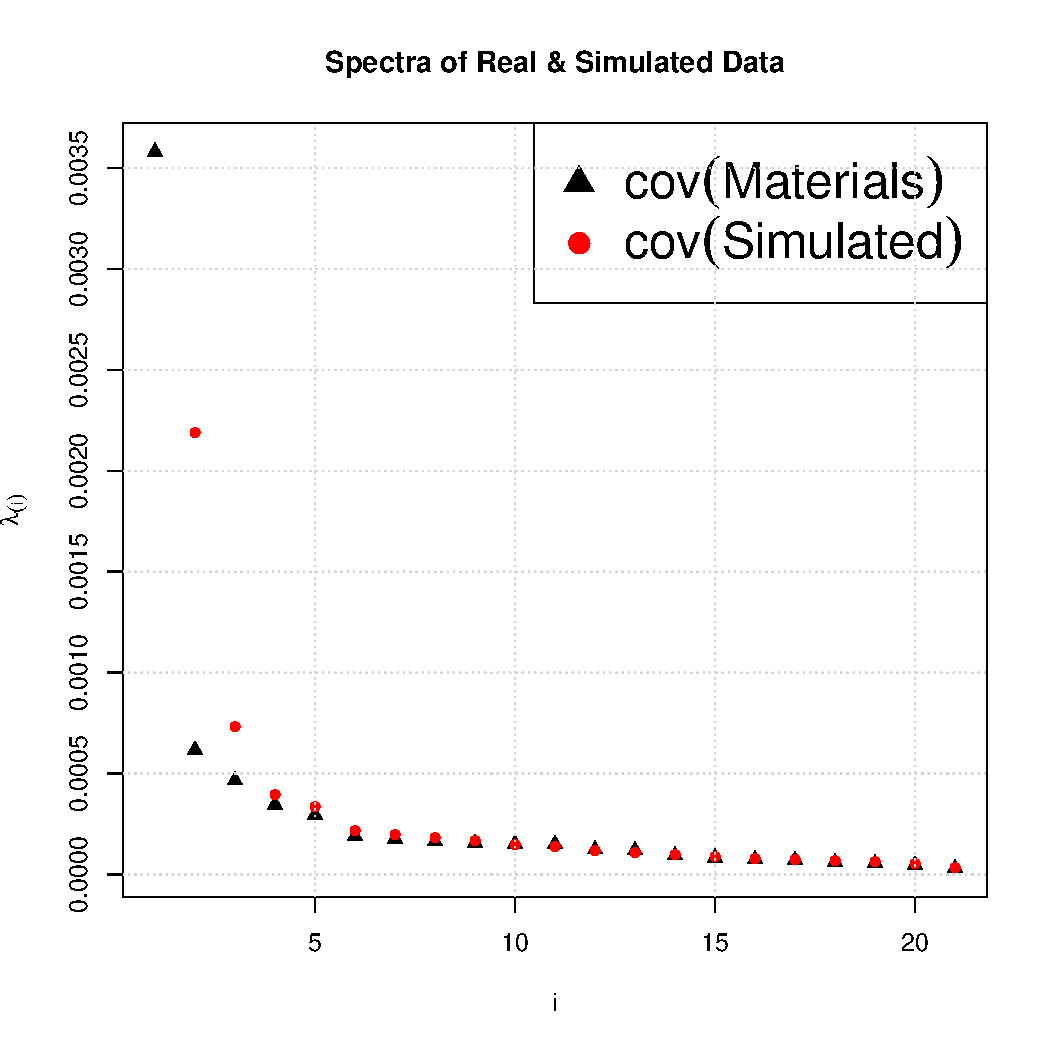
\includegraphics[scale=0.6]{Materials_eigenvalues.pdf}
  \caption{Eigenvalues of Materials: real \& simulated}
  \label{fig:Materials_eigenvalues}
\end{figure}

\begin{figure}[htb!]
  \centering
  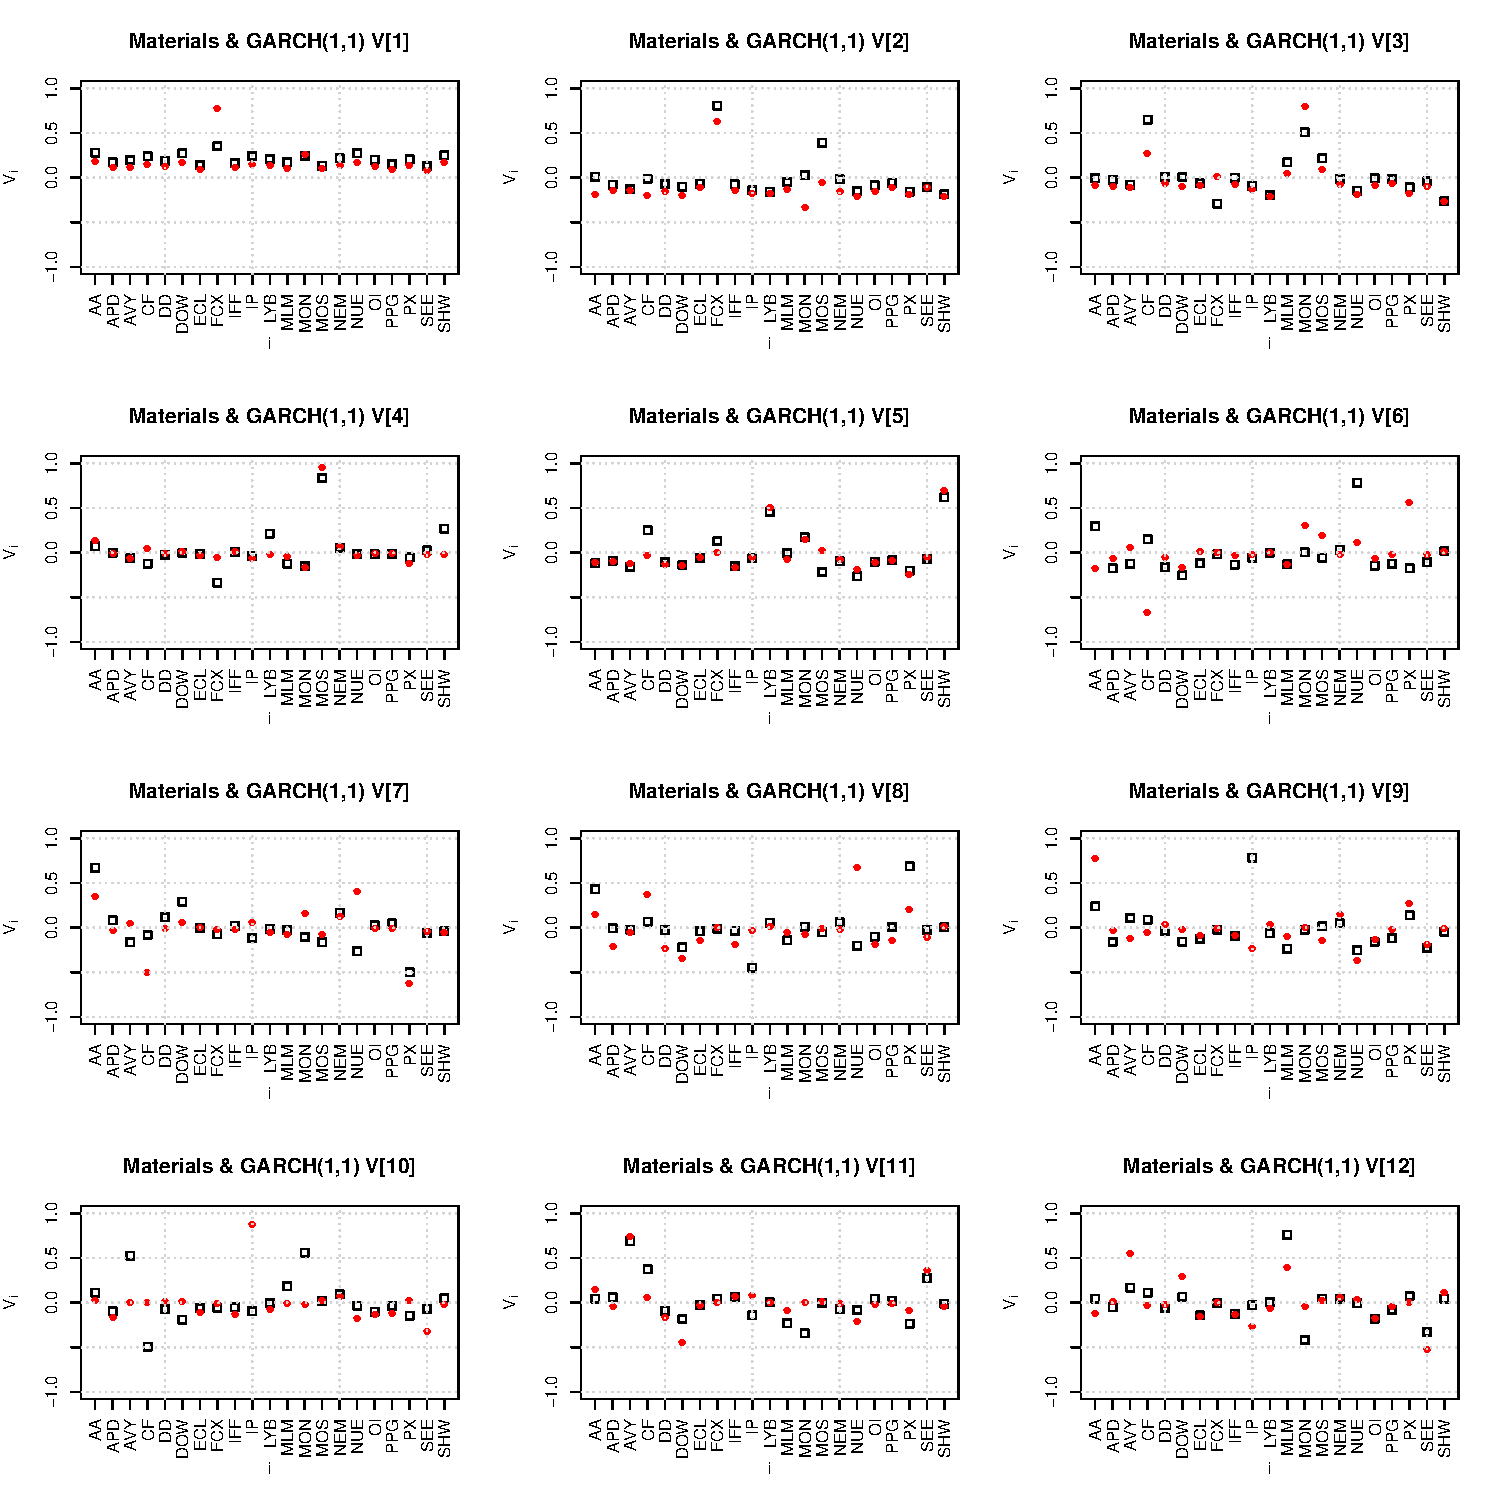
\includegraphics[scale=0.5]{Materials_eigenvectors1.pdf}
  \caption{Eigenvectors of Materials: real \& simulated}
  \label{fig:Materials_eigenvectors1}
\end{figure}

\begin{figure}[htb!]
  \centering
  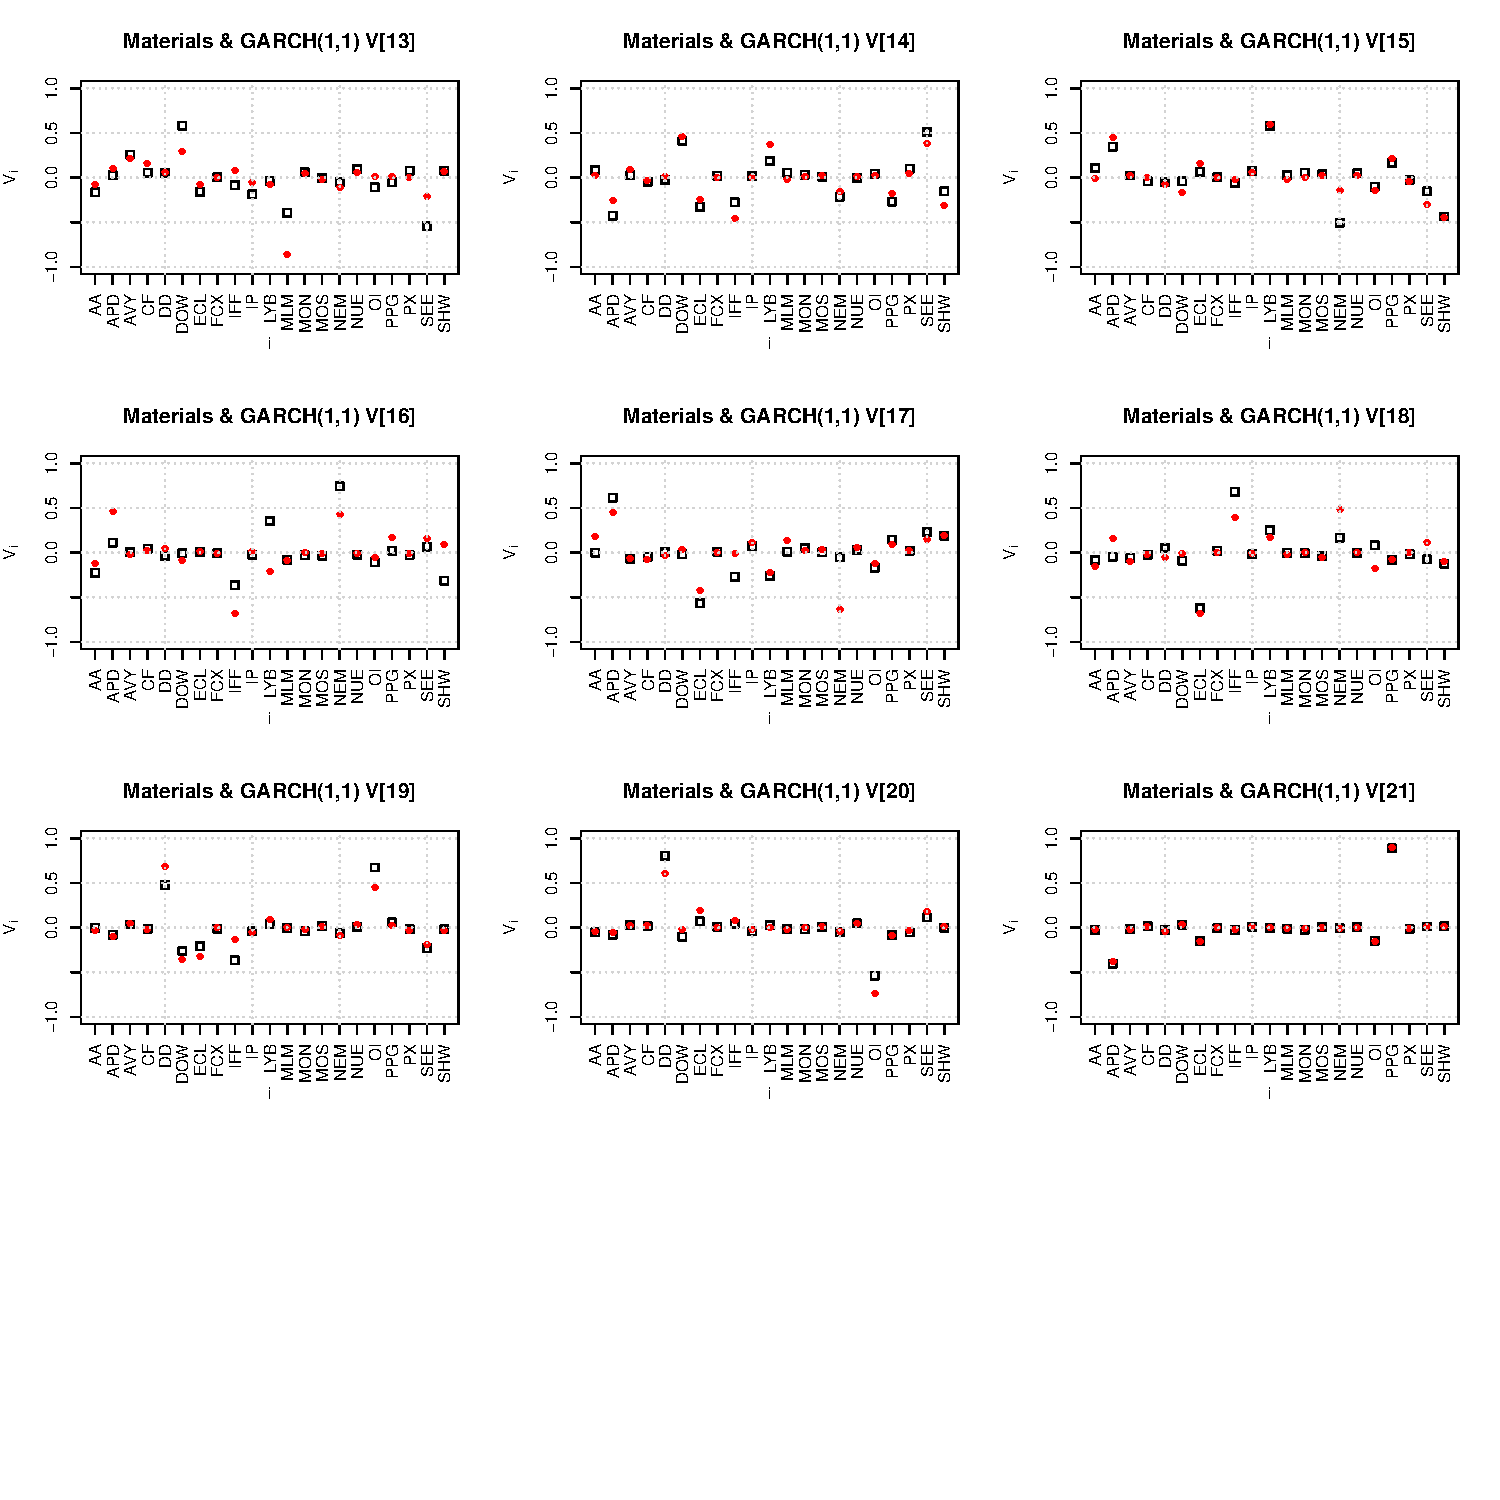
\includegraphics[scale=0.5]{Materials_eigenvectors2.pdf}
  \caption{Eigenvectors of Materials: real \& simulated continued}
  \label{fig:Materials_eigenvectors2}
\end{figure}

\bibliographystyle{unsrt}
\bibliography{../thesis/econophysics}
\end{document}
